\documentclass[11pt, a4paper]{article}
\usepackage[utf8]{inputenc} % comment when using lualatex
\usepackage{fullpage}
\usepackage{graphicx}
\usepackage[hidelinks]{hyperref,xcolor}
\renewcommand\UrlFont{\color{blue}\rmfamily}

% Bibliography management
%  see https://www.overleaf.com/learn/latex/Biblatex_citation_styles
%  and https://www.overleaf.com/learn/latex/Bibliography_management_in_LaTeX
% to use overleaf with reference manager
%  see: https://no.overleaf.com/blog/639-tip-of-the-week-overleaf-and-reference-managers
% \usepackage[backend=biber]{biblatex}
% \addbibresource{library.bib} %Imports bibliography file
 
% Title of your project
\title{Torque in a Variable Reluctance Machine}

% Name of deliverable
\newcommand{\deliverableName}{Selected Topics on Electrical Machines}

% Group names(s)
\author{Yusuf \textsc{KOSESOY}\\ e2483394}

% Group number
\newcommand{\groupNumber}{x}

% Any comments for us
\newcommand{\comments}{Project 1}

 % Web address for the project (if any)
\newcommand{\homepage}{\url{http://keysan.me/ee568/}}

% Date for title page, default is today and 
\date{\today~(Spring 2020)}


\makeatletter{}

\begin{document}

% Title page based on https://www.latextemplates.com/template/academic-title-page
\begin{titlepage}
  	\newcommand{\HRule}{\rule{\linewidth}{0.3mm}} % Defines a new command for horizontal lines, change thickness here
	\center % Centre everything on the page
	%------------------------------------------------
	%	Headings
	%------------------------------------------------
	
	\textsc{\LARGE Middle East Technical University}\\[1.5cm]
	
	\textsc{\Large EE568 - \deliverableName}\\[0.5cm]
	
	\textsc{\large Electrical Electronics Engineering}\\[0.5cm]
	
	%------------------------------------------------
	%	Title
	%------------------------------------------------
	
	\HRule\\[0.4cm]
	
	{\huge\bfseries \@title}\\[0.4cm]
	
	\HRule\\[1.5cm]
	
	%------------------------------------------------
	%	Author(s)
	%------------------------------------------------
	\begin{minipage}{0.4\textwidth}
		\begin{flushleft}
			\large
			\textit{}\\
			\@author % Your name
		\end{flushleft}
	\end{minipage}
	~
	\begin{minipage}{0.4\textwidth}
		\begin{flushright}
			\large
			\textit{}
		\end{flushright}
	\end{minipage}
	
% 	If you don't want a supervisor, uncomment the two lines below and comment the code above
% 	{\large\textit{Author(s)}}\\
% 	\@author % Your name
	
	%------------------------------------------------
	%	Date
	%------------------------------------------------
	
	\vfill\vfill
		{\large\@date} % Date, change the \today to a set date if you want to be precise
    \vfill\vfill\vfill
	
    \footnotesize{ \comments}
    \vfill\vfill
    \homepage
    \vfill
    
    %------------------------------------------------
    % Change log for the plan (can be deleted before delivery)
    % When you update the plan please record what you changed and what the reason for the change. This will be useful for your supervisor.
    %------------------------------------------------
    % \begin{tabular}{ | l | l | l | l |}
    \hline
    \textbf{Version} & \textbf{Date of change} & \textbf{What is changed?} & \textbf{The reason for the change} \\ \hline
    0.1 & 03-10-2010 & first version & \\
    \hline
\end{tabular}
	
	%------------------------------------------------
	%	Logo
	%------------------------------------------------
	\vfill
	
\includegraphics[width=0.5\textwidth]{figures/Odtu-metu-logo.png}
	\vfill
	 
	
\end{titlepage}


\section*{Introduction}

Reluctance, inductance and torque equations are derived as analytical model for variable reluctance motor in this report. The results of the analytical model were obtained with the help of MATLAB. Finite element analysis (FEA) is carried out for given parameters and results are compared with analytical results. FEMM is used for FEA. Bonus questions are also tried to be handled.
FEA is carried out for both linear and non-linear material. Their effect on model is observed and discussed. Saturating and fringing is observed in analysis.



\subsection*{Question 1}
\subsubsection*{a)}

Since core permeability ($\mu_r$) is assumed to be infinite, reluctance of core is zero, as it can be easily calculated in Eq-\ref{reluctance} where $l$ is length, $\mu$ is permeability and $A$ is cross section area. Therefore, total reluctance of flux path comes into existence only because of air-gaps. There are two air-gaps around rotor. In this report, each length of air-gap is called 'g' and the depth of core is called 'h'. To calculated reluctance of air gap, cross section area of flux path needs to be evaluated. The area is function of angle to stator which rotor has.

\begin{equation}
\label{reluctance}
\mathcal{R}=\frac{l}{\mu_r  \mu_0  A}
\end{equation} \\
Flux flows through over more permeable path. Flux chooses the path which has 0.5 mm air-gap until certain angle that calculated as asin(7.5/12.5). Because of rotor geometry, air-gap is 2.5 mm from asin(7.5/12.5) to acos(7.5/12.5). The certain angle is obtained with help of Fig-\ref{aci_hesabi}. Accordingly, reluctance needs to be defined as partial function.\\

For this system, $l$ is $2g$ and $A$ can be obtained with Eq-\ref{cross_section} and generalized function of reluctance is given in Eq-\ref{genel_reluctance}. $h$ is already given as 20 mm. When $\alpha$ is  smaller than  asin(7.5/12.5), $r$ is 12 mm and $g$ is 0.5 mm, but when $\alpha$ is between asin(7.5/12.5) and acos(7.5/12.5), $r$ is 10 mm and $g$ is 2.5 mm.\\

%FIGURE
\begin{figure}[ht]
\centering
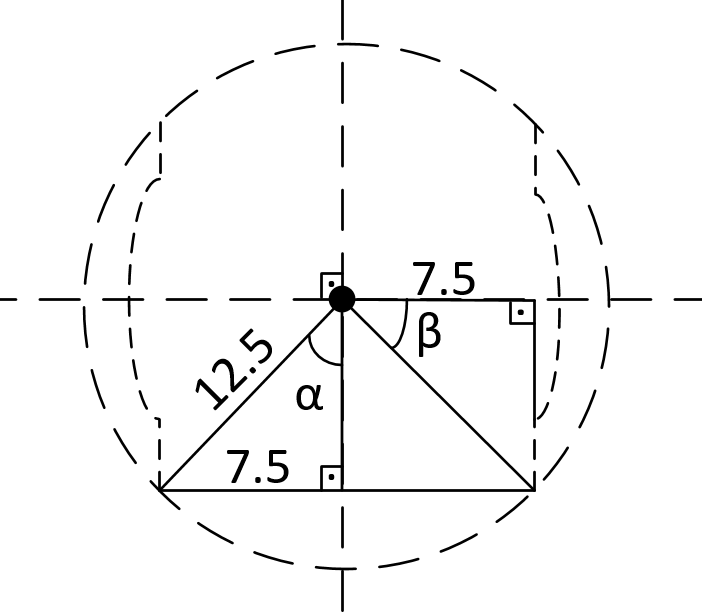
\includegraphics[width=0.5\textwidth]{figures/angle_calculation.PNG}
\caption{The certain angle that changes air-gap length } \label{aci_hesabi}
\end{figure}

\begin{equation}
\label{cross_section}
A=h(r+0.5g)\alpha
\end{equation}

\begin{equation}
\label{genel_reluctance}
\mathcal{R}=\frac{2g}{\mu_r  h (r+0.5g) \alpha}
\end{equation} \\

Inductance is function of reluctance and number of turn. The relationship between them is given in Eq-\ref{inductance}. If Eq-\ref{genel_reluctance} is placed into Eq-\ref{inductance}, Eq-\ref{inductance_func} is derived as a function of $\alpha$. 

\begin{equation}
\label{inductance}
L=\frac{N^2}{\mathcal{R}}
\end{equation} 

\begin{equation}
\label{inductance_func}
L(\alpha)=\frac{\mu_0 N^2 h (r+0.5g) \alpha}{2g}
\end{equation}

%FIGURE
\begin{figure}[ht]
\centering
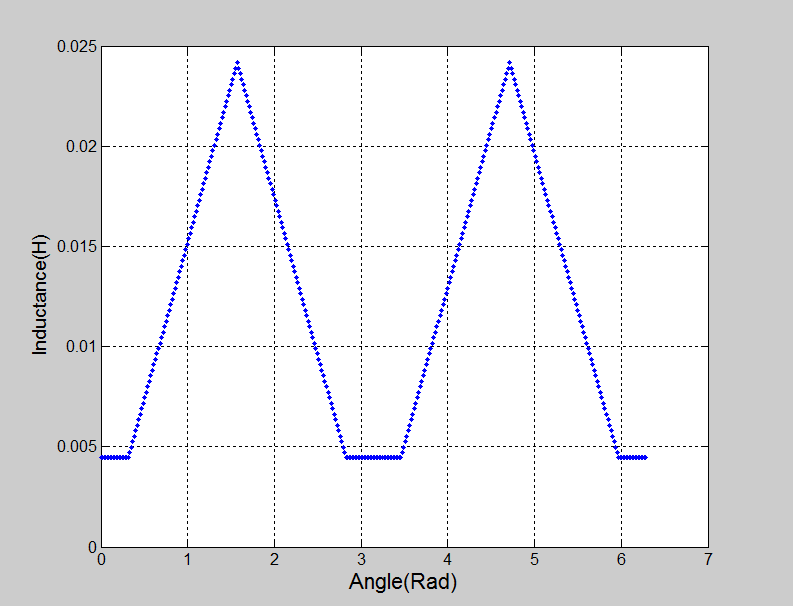
\includegraphics[width=0.7\textwidth]{figures/inductance_graph.PNG}
\caption{Inductance as function rotation } \label{inductance_graph}
\end{figure}

Inductance is plotted as a function of rotational angle in Fig-\ref{inductance_graph}. Unit of angle is radian. It is observable that inductance is increasing while air-gap is getting smaller and decreasing while air-gap is getting larger linearly. It is inversely proportional to reluctance.\\

Initial position of rotor is determined as perfectly aligned to core. Therefore, inductance has its lowest value roughly as 0.005H at first and last 26$^\circ$ of 180$^\circ$ period. Its peak value is almost 0.025H. Derivative of increasing and decreasing of inductance is equal and constant as it can be calculated.

\subsubsection*{b)}

Torque is given in Eq-\ref{torque_general}. If Eq-\ref{inductance_func} is placed in the Eq-\ref{torque_general}, torque equality is obtained as shown in Eq-\ref{torque_spec}. Generated torque as a function of rotation is plotted in Fig-\ref{torque_graph}. It can also be verified by using inductance as a function of rotation which is plotted in Fig-\ref{inductance_graph}. There is ratio between inductance and generated torque which can be observable in Eq-\ref{torque_general}. Since derivation of inductance is constant, generated torque is constant as well.

\begin{equation}
\label{torque_general}
T=\frac{1}{2} i^2 \frac{dL(\alpha)}{d \alpha}
\end{equation} 

\begin{equation}
\label{torque_spec}
T=\frac{\mu_0 N^2 i^2 h (r+0.5g)}{4g}
\end{equation} 

%FIGURE
\begin{figure}[ht]
\centering
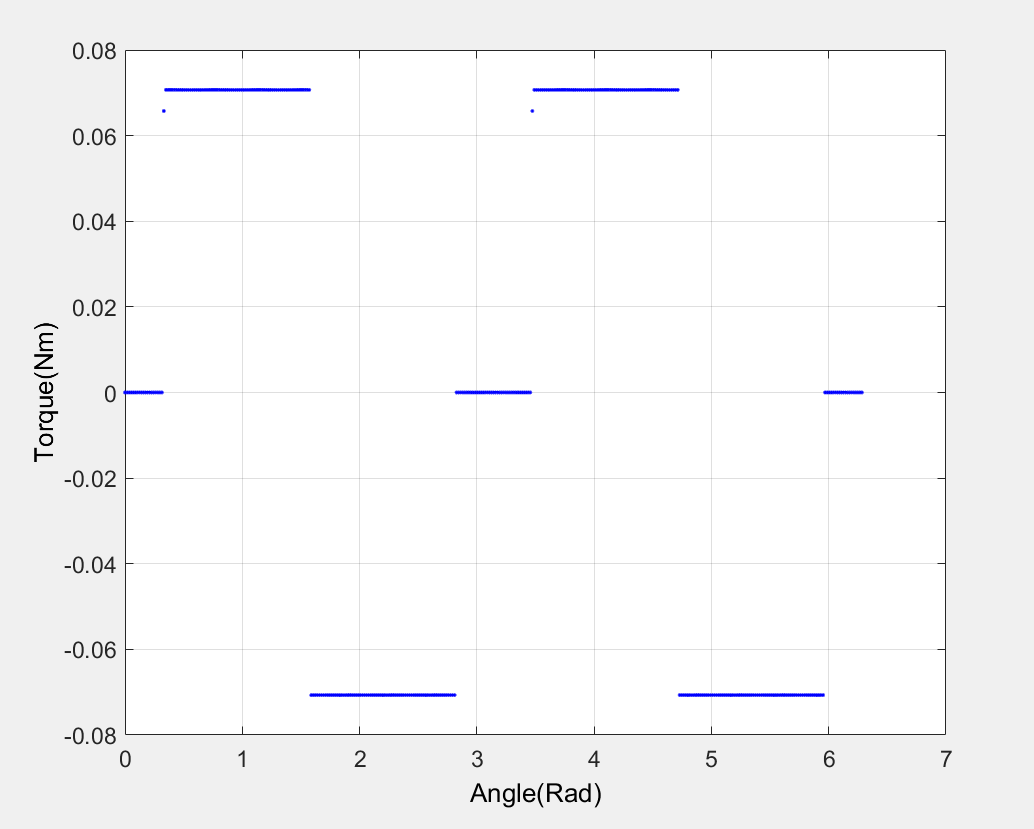
\includegraphics[width=0.7\textwidth]{figures/torque_graph.PNG}
\caption{Torque as function rotation } \label{torque_graph}
\end{figure}


\subsubsection*{c)}

System model can be more accurate, if non-linearity and losses are considered while calculations are carried on. Core losses can be included as a parameter which can effect other critical system parameters such as inductance and relatively torque by causing heat and making changes on B-H curve. \\

Core lamination is another point which can be considered as a solution to non-homogeneous flux distribution. By avoiding this issue, it also helps to reduce core losses since lamination prevents eddy current and its impact, therefore heat does not increase and non-linearize the B-H curve. \\

There could be a predefined ratio between air-gap and core cross section area to include fringing effects to analytical model. The system is assumed ideal at some points which also includes that there is no fringing flux, but it is an effect that takes modeling away from accuracy.

\subsection*{Question 2}

\subsubsection*{a)}

Flux density vectors for 0$^\circ$, 45$^\circ$ and 90$^\circ$ in Fig-\ref{Lin_0}, Fig-\ref{Lin_45} and Fig-\ref{Lin_90}, respectively for linear core material. FEMM is used to perform FEA. It has 2D modeling interface. Despite its limited abilities, it takes short time to perform analysis and does not tire computer.\\

Core material is selected as M-15 steel from FEMM material library. It can carry up to 1T magnetic flux density. FEA measures 1.1T for its maximum inductance value. \\

\begin{figure}[ht]
\centering
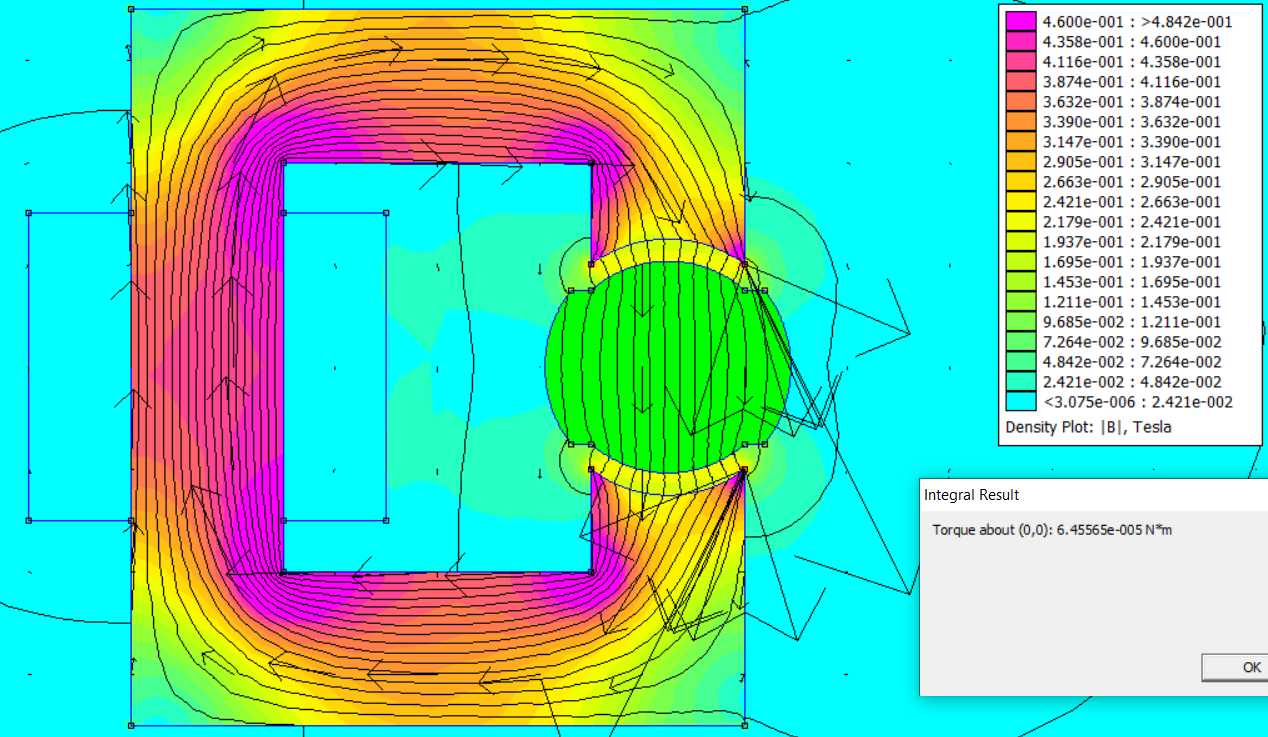
\includegraphics[width=0.8\textwidth]{figures/Lin_0.PNG}
\caption{Magnetic flux density vectors for linear core material at $\alpha$=0 } \label{Lin_0}
\end{figure}

\begin{figure}[ht]
\centering
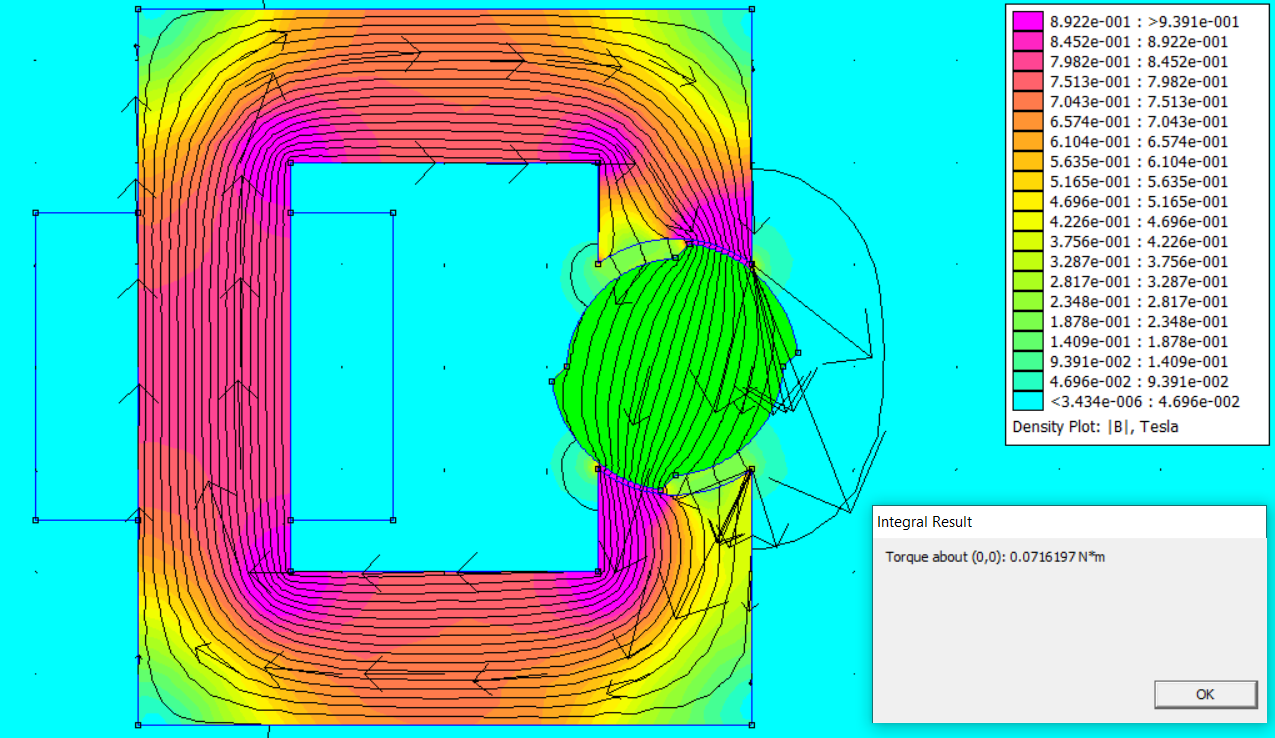
\includegraphics[width=0.8\textwidth]{figures/Lin_45.PNG}
\caption{Magnetic flux density vectors for linear core material at $\alpha$=45 } \label{Lin_45}
\end{figure}

\begin{figure}[ht]
\centering
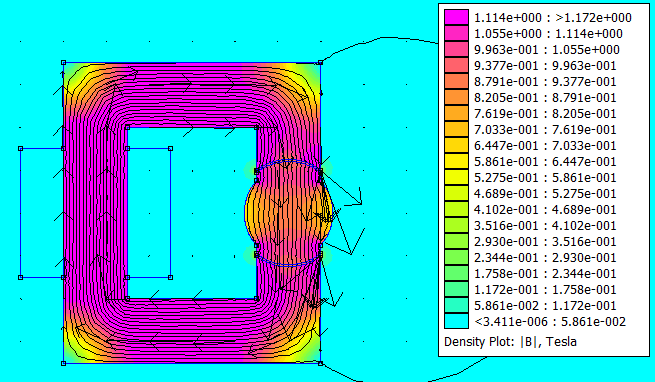
\includegraphics[width=0.8\textwidth]{figures/Lin_90.PNG}
\caption{Magnetic flux density vectors for linear core material at $\alpha$=90 } \label{Lin_90}
\end{figure}



\subsubsection*{b)}

Inductance is measured by FEMM in unit of Henry(H) at three different position, 0$^\circ$, 45$^\circ$ and 90$^\circ$. Results are given in Table \ref{tab:linear_in_en}. FEA results verifies the analytical results with low error rate. Error might also be due to core reluctance since permeability of core is assumed infinite for analytical calculations.\\

Stored energy in the system is also measured by using FEA and presented in Table-\ref{tab:linear_in_en}. Stored energy is directly proportional to inductance, therefore it is expected to have three times stored energy at $\alpha$=0$^\circ$ of energy stored at $\alpha$=90$^\circ$ since the inductance is tripled. Stored energy is very close to what it should be and it can be said that core saturates for only 0.1T depending on the results in Fig-\ref{Lin_90} and Table-\ref{tab:linear_in_en}, for this reason there is only a small error. Core could be defined as totally linear, but saturation after constant permeability would not be visible and it is not realistic. 

\begin{equation}
\label{Energy}
\mathcal{W}=\frac{1}{2}i^2 L(\alpha)
\end{equation} 

%TABLE
\begin{table}[ht]
\centering
\caption{Inductance and energy for linear material} 
\begin{tabular}[t]{lrr}
\hline
Rotational Position        & Inductance(H) & Stored Energy(J)  \\
\hline
0$^\circ$     & 0.0103       & 0.0467     \\
45$^\circ$    & 0.0200       & 0.0901     \\
90$^\circ$    & 0.0305       & 1.1359       \\
\hline
\end{tabular}
\label{tab:linear_in_en}
\end{table}


\subsubsection*{c)}

Applied torque to the rotor is calculated by using FEA and analytical model. Results are close enough to be accepted, but there is a conflict at exact 90$^\circ$. That conflict disappears at very close angles to the 90$^\circ$ like 85$^\circ$. The results are given in Table-\ref{tab:linear_tor}. The reason of this situation is magnetic behaviour of system at 90$^\circ$ is not defined in analytical model. Torque calculation in analytical model depends on the inductance difference per degree, but magnetic behavior at 90$^\circ$ does not generate inductance difference.

%TABLE
\begin{table}[ht]
\centering
\caption{Torque for linear material} 
\begin{tabular}[t]{c|r r}
\hline
Rotational Position & \multicolumn{2}{c}{Torque(Nm)}\\
\cline{2-3}
                           & FEA         & Analytical \\
\hline
0$^\circ$     & 0.00006     & 0          \\
45$^\circ$    & 0.0716      & 0.707      \\
85$^\circ$    & 0.0601      & 0.707      \\
90$^\circ$    & 0.0.0013    & 0.707          \\
\hline
\end{tabular}
\label{tab:linear_tor}
\end{table}

\subsection*{Question 3}
\subsubsection*{a)}

 Core material is selected as soft magnetic composition (Fe, Ni, Zn, V) from FEMM material library. It can carry up to 0.1T magnetic flux density.  FEA measures 0.32T for its maximum inductance value. Flux density vectors for 0$^\circ$, 45$^\circ$ and 90$^\circ$ in Fig-7, Fig-8 and Fig-9, respectively for nonlinear core material.\\
 
 Core material saturates, therefore energy can not be stored and converted into applied torque to the rotor.

\begin{figure}[ht]
\centering
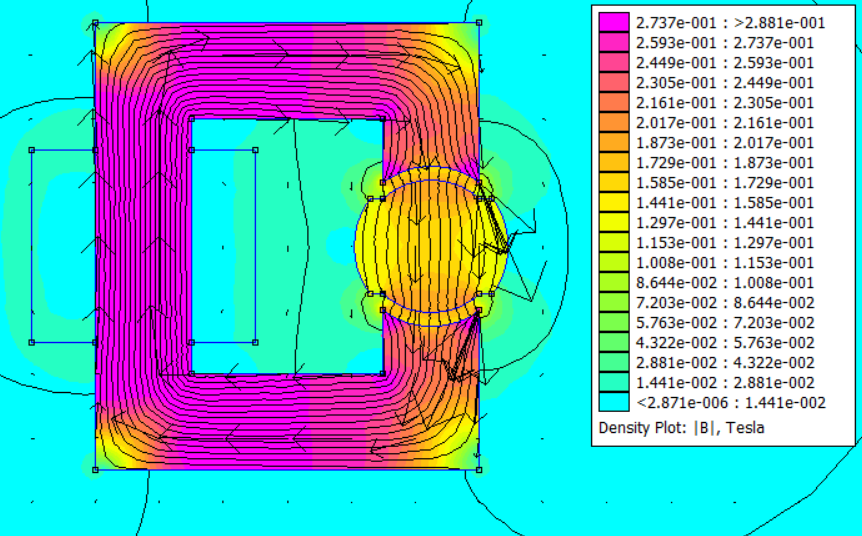
\includegraphics[width=0.9\textwidth]{figures/Non_0.PNG}
\caption{Magnetic flux density vectors for linear core material at $\alpha$=0 } \label{Non_0}
\end{figure}

\begin{figure}[ht]
\centering
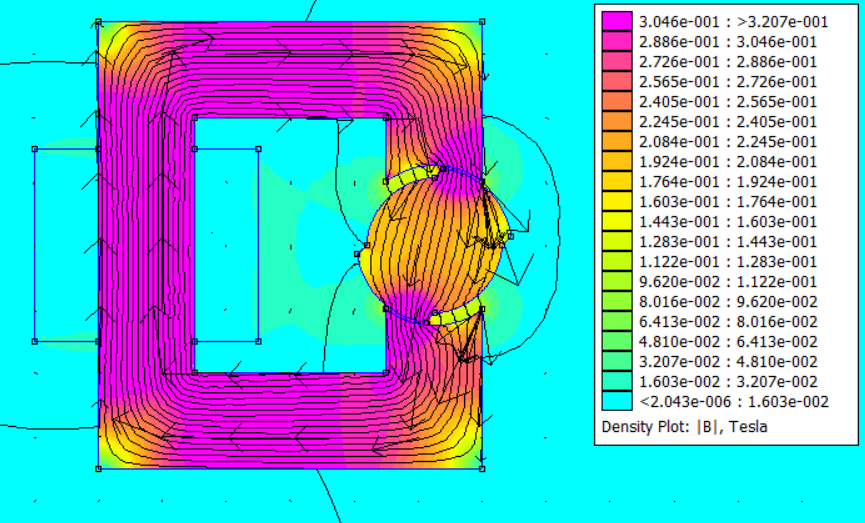
\includegraphics[width=0.9\textwidth]{figures/Non_45.PNG}
\caption{Magnetic flux density vectors for nonlinear core material at $\alpha$=45 } \label{Non_45}
\end{figure}

\begin{figure}[ht]
\centering
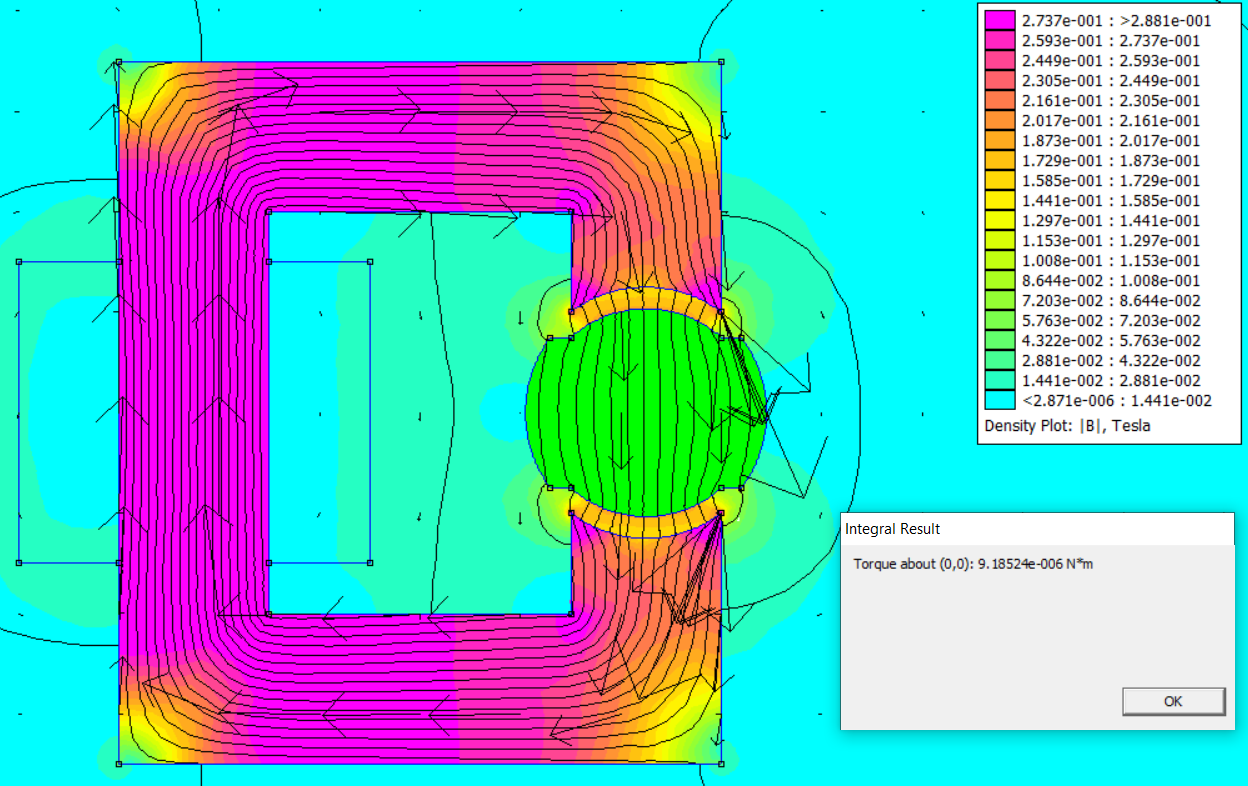
\includegraphics[width=0.9\textwidth]{figures/Non_90.PNG}
\caption{Magnetic flux density vectors for nonlinear core material at $\alpha$=90 } \label{Non_90}
\end{figure}

\subsubsection*{b)}

Analytical results of inductance and stored energy do not match up with FEA results, because analytical method is based on linear core material and the core has nonlinear B-H curve. In other words, permeability of core is not constant. FEA results are give in Table-\ref{tab:nonlinear_in_en}.

%TABLE
\begin{table}[ht]
\centering
\caption{Inductance and energy for nonlinear material} 
\begin{tabular}[t]{lrr}
\hline
Rotational Position        & Inductance(H) & Stored Energy(J)  \\
\hline
0$^\circ$     & 0.0082       & 0.0323     \\
45$^\circ$    & 0.0089       & 0.0248     \\
90$^\circ$    & 0.0093       & 0.0203     \\
\hline
\end{tabular}
\label{tab:nonlinear_in_en}
\end{table}

\subsubsection*{c)}

Analytical results do not match up with FEA results for torque values as well. Reasons for this situation is same as the reasons mentioned in a and b parts. FEA results are give in Table-\ref{tab:nonlinear_tor}.

%TABLE
\begin{table}[ht]
\centering
\caption{Torque for linear material} 
\begin{tabular}[t]{lrr}
\hline
Rotational Position        & Torque(Nm)  \\
\hline
0$^\circ$     & 0.000008           \\
45$^\circ$    & 0.0185            \\
90$^\circ$    & 0.0.00008              \\
\hline
\end{tabular}
\label{tab:nonlinear_tor}
\end{table}

\subsubsection*{d)}

Based on the results presented in the report, inductance and relatively reluctance formula which are given in Eq-\ref{inductance_func} and Eq-\ref{reluctance}, respectively, does not  have a parameter of current. It may seem like there is no effect of amplitude of current to inductance, but if the amplitude of current generated  magnetic flux more than core can carry, saturation occurs and inductor would not be able to behave as inductance value. Correspondingly, less energy is stored and relatively less torque is generated. Non saturating system result are given in Table-\ref{tab:linear_in_en}, when there is saturating system results are given in Table-\ref{tab:nonlinear_in_en} for same current amplitude. Obviously, saturating effects inductance and torque negatively.\\

Some magnetic flux vectors travel over longer path in the air-gap to reach the core again. This increases the reluctance and proportionally decreases the inductance. Larger air-gap means more fringing flux which can be observable in Fig-\ref{Lin_0} and Fig-\ref{Lin_90}.\\

Saturation also limits the magnetic flux density carried on the core. Saturating systems have less magnetic field density and consequently less fringing flux compared to non saturating systems. This can be observable by examining Fig-\ref{Lin_90} and Fig-\ref{Non_90}.

\subsection*{Question 4}

Generated torque equation is given in Eq-\ref{torque_general}. Square of current is always positive, therefore derivative of inductance needs to be positive. In other words, inductance needs to increase at specified degree interval. In Fig-\ref{torque_graph}, there is an obvious positive torque value and Fig-\ref{inductance_graph} is indicator of increasing inductance. Generated positive torque in the 2D model is given in Fig-\ref{positive_torque} as it is 0.0717 Nm.

\begin{figure}[ht]
\centering
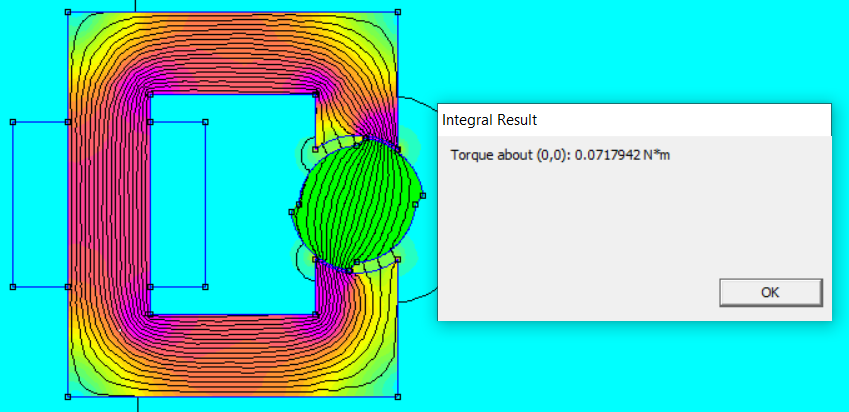
\includegraphics[width=0.9\textwidth]{figures/positive_torque_1.PNG}
\caption{Generated torque in 2D model} 
\label{positive_torque}
\end{figure}

\subsection*{Question 5}

There is an animation of physical motion of the model on GitHub, but flux density variation is not visible because the author of this report is newbie on Maxwell platform.

\subsection*{Question 6}

The system is modelled in Maxwell 3D platform and angle of rotation is defined as parametric. The inductance value is measured at each 5$^\circ$ of 360$^\circ$. Results are given in Fig-\ref{maxwell_inductance}.\\

Lowest value of inductance does not match with analytical results and 2D model results. The reason for this situation might be the core material selection. In 3D model, cobalt is selected as core material.

\begin{figure}[ht]
\centering
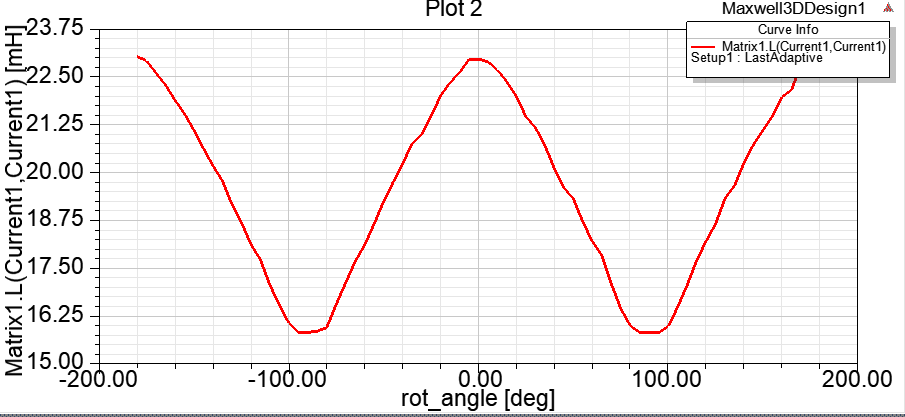
\includegraphics[width=0.9\textwidth]{figures/maxwell_inductance.PNG}
\caption{Inductance as function of rotation plotted on 3D Maxwell} 
\label{maxwell_inductance}
\end{figure}


%References
%\printbibliography 




\end{document}
